\documentclass[a4paper]{article}

\usepackage{INTERSPEECH2016}

\usepackage{graphicx}
\usepackage{amssymb,amsmath,bm}
\usepackage{textcomp}

\def\vec#1{\ensuremath{\bm{{#1}}}}
\def\mat#1{\vec{#1}}


\sloppy % better line breaks
\ninept

\title{Paper Template for INTERSPEECH 2016}

%%%%%%%%%%%%%%%%%%%%%%%%%%%%%%%%%%%%%%%%%%%%%%%%%%%%%%%%%%%%%%%%%%%%%%%%%%
%% If multiple authors, uncomment and edit the lines shown below.       %%
%% Note that each line must be emphasized {\em } by itself.             %%
%% (by Stephen Martucci, author of spconf.sty).                         %%
%%%%%%%%%%%%%%%%%%%%%%%%%%%%%%%%%%%%%%%%%%%%%%%%%%%%%%%%%%%%%%%%%%%%%%%%%%
%\makeatletter
%\def\name#1{\gdef\@name{#1\\}}
%\makeatother
%\name{{\em Firstname1 Lastname1, Firstname2 Lastname2, Firstname3 Lastname3,}\\
%      {\em Firstname4 Lastname4, Firstname5 Lastname5, Firstname6 Lastname6,
%      Firstname7 Lastname7}}
%%%%%%%%%%%%%%% End of required multiple authors changes %%%%%%%%%%%%%%%%%

\makeatletter
\def\name#1{\gdef\@name{#1\\}}
\makeatother \name{{\em Author Name$^1$, Co-author Name$^2$}}

\address{$^1$Author Affiliation \\
  $^2$Co-author Affiliation \\
  {\small \tt author@university.edu, coauthor@company.com}
}

%\twoauthors{Karen Sp\"{a}rck Jones.}{Department of Speech and Hearing \\
%  Brittania University, Ambridge, Voiceland \\
%  {\small \tt Karen@sh.brittania.edu} }
%  {Rose Tyler}{Department of Linguistics \\
%  University of Speechcity, Speechland \\
%  {\small \tt RTyler@ling.speech.edu} }

%
\begin{document}

  \maketitle
  %
  \begin{abstract}
    This is the layout specification and template definition for the INTERSPEECH 2016 Conference, which will be held in San Francisco, California during September 8-12, 2016.
    This template has been generated from previous INTERSPEECH templates. 
    The format is essentially the one used for IEEE ICASSP conferences. 
    The maximum number of pages is 5. 
    The 5\textsuperscript{th} page may be used exclusively for references. 
    Index terms should be included as shown below.
  \end{abstract}
  \noindent{\bf Index Terms}: speech recognition, human-computer interaction, computational paralinguistics



  \section{Introduction}

    This template can be found on the conference website.
    Templates are provided for LibreOffice, Microsoft Word\textregistered, and \LaTeX.
    However, we highly recommend using \LaTeX\ when preparing your submission.     
    Information for full paper submission is available on the conference website.

  
  \section{Page layout and style}

    Authors should observe the following rules for page layout. 
    A highly recommended way to meet these requirements is to use a given template (LibreOffice, Microsoft Word\textregistered\ or \LaTeX) and check details against the corresponding example PDF file.
    Given templates, Microsoft Word\textregistered\ or \LaTeX, can be adapted/imported easily in other software such as LibreOffice, Apple Pages, Lua\LaTeX, and Xe\LaTeX, but please be careful to match the layout of the provided PDF example.  
    \subsection{Basic layout features}

      \begin{itemize}
        \item Proceedings will be printed in DIN~A4 format. Authors must submit their papers in DIN~A4 format.
        \item Two columns are used except for the title part and possibly for large figures that need a full page width.
        \item Left and right margin are 20\,mm each.
        \item Column width is 80\,mm.
        \item Spacing between columns is 10\,mm.
        \item Top margin 25\,mm (except for the first page which is 30\,mm to the title top).
        \item Bottom margin is 35\,mm.
        \item Text height (without headers and footers) is maximum 235\,mm.
        \item Headers and footers must be left empty. They will be added for printing and the INTERSPEECH 2016 media.
        \item Check indentations and spacings by comparing to this example file (in PDF).
      \end{itemize}


      \subsubsection{Headings}

        Section headings are centered in boldface with the first word capitalized and the rest of the heading in lower case.
        Sub-headings appear like major headings, except they start at the left margin in the column.
        Sub-sub-headings appear like sub-headings, except they are in italics and not boldface. 
        See the examples given in this file. 
        No more than 3 levels of headings should be used.

  
    \subsection{Text font}

      Times or Times Roman font is used for the main text. 
      Font size in the main text must be 9 points, and in the References section 8 points. 
      Other font types may be used if needed for special purposes. 
      It is VERY IMPORTANT that while making the final PDF file, you embed all used fonts!

      \LaTeX\ users: users should use Adobe Type~1 fonts such as Times or Times Roman. 
      These are used automatically by the INTERSPEECH2016.sty style file. 
      Authors must not use Type~3 (bitmap) fonts.

  
    \subsection{Figures}

      All figures must be centered on the column (or page, if the figure spans both columns).
      Figure captions should follow each figure and have the format given in Figure~\ref{fig:speech_production}.

      Figures should preferably be line drawings. 
      If they contain gray levels or colors, they should be checked to print well on a high-quality non-color laser printer.

      Graphics (i.\,e., illustrations, figures) must not use stipple fill patterns because they will not reproduce properly in Adobe PDF.
      Please use only SOLID FILL COLORS.

      Figures which span 2 columns (i.\,e., occupy full page width) should be placed at the top or bottom of the page.


    \subsection{Tables}

      An example of a table is shown as Table \ref{tab:example}. 
      The caption text may be above or below the table.

      \begin{table}[th]
        \caption{\label{tab:example} {\it This is an example of a table.}}
        \vspace{2mm}
        \centerline{
          \begin{tabular}{| r@{}l | r |}
            \hline
            \multicolumn{2}{|c|}{ratio} & 
            \multicolumn{1}{c|}{decibels} \\
            \hline \hline
               $1$ & $/10$&       $-20$~~~ \\
               $1$ & $/1$ &         $0$~~~ \\
               $2$ & $/1$ & $\approx 6$~~~ \\
            $3.16$ & $/1$ &        $10$~~~ \\
              $10$ & $/1$ &        $20$~~~ \\
             $100$ & $/1$ &        $40$~~~ \\
            $1000$ & $/1$ &        $60$~~~ \\
            \hline
          \end{tabular}
        }
      \end{table}

  
    \subsection{Equations}

      Equations should be placed on separate lines and numbered. 
      Examples of equations are given below.
      Particularly,
      %
      \begin{equation}
        x(t) = s(f_\omega(t))
        \label{eq1}
      \end{equation}
      %
      where \(f_\omega(t)\) is a special warping function
      %
      \begin{equation}
        f_\omega(t) = \frac{1}{2 \pi j} \oint_C 
        \frac{\nu^{-1k} \mathrm{d} \nu}
             {(1-\beta\nu^{-1})(\nu^{-1}-\beta)}
        \label{eq2}
      \end{equation}
      %
      A residue theorem states that
      %
      \begin{equation}
        \oint_C F(z)\,\mathrm{d}z = 2 \pi j \sum_k \mathrm{Res}[F(z),p_k]
        \label{eq3}
      \end{equation}
      %
      Applying (\ref{eq3}) to (\ref{eq1}), it is straightforward to see that
      %
      \begin{equation}
        1 + 1 = \pi
        \label{eq4}
      \end{equation}

      Finally we have proven the secret theorem of all speech sciences.
      No more math is needed to show how useful the result is!

      \begin{figure}[t]
        \centering
        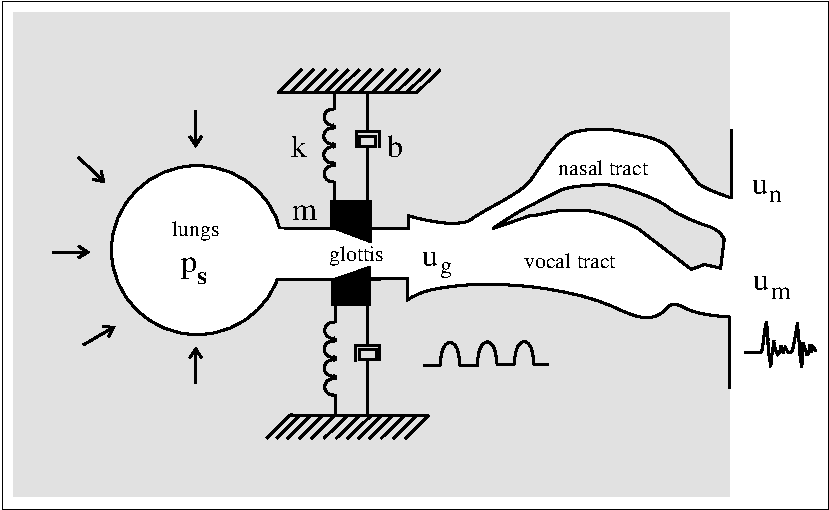
\includegraphics[width=\linewidth]{figure.pdf}
        \caption{{\it Schematic diagram of speech production.}}
        \label{fig:speech_production}
      \end{figure}
  
      Proper typesetting helps to understand the content faster.
      The preferred way of printing vectors and matrices is:
      %
      \begin{equation}
        \vec{x}_i,~\vec{\alpha},~\mat{X}
      \end{equation}

  
    \subsection{Hyperlinks}

      For technical reasons, the proceedings editor will strip all active links from the papers during processing. 
      Hyperlinks can be included in your paper, if written in full, e.\,g.\ ``http://www.foo.com/index.html''.
      The link text must be all black. 
      Please make sure that they present no problems in printing to paper.

  
    \subsection{Multimedia files}

      The INTERSPEECH 2016 organizing committee offers the possibility to submit multimedia files. 
      These files are meant for audio-visual illustrations that cannot be conveyed in text, tables and graphs.
      Just like you would when including graphics, make sure that you have sufficient author rights to the multimedia materials that you submit for publication. 
      The proceeding media will NOT contain readers or players, so be sure to use widely accepted file formats, such as MPEG, Windows WAVE PCM (.wav) or Windows Media Video (.wmv) using standard codecs.
      The files you submit will be accessible from the abstract cards on the media and via a bookmark in the manuscript.
      From within the manuscript, refer to a multimedia illustration by its filename. Use short file names without blanks.

  
    \subsection{Page numbering}

      Final page numbers will be added later to the document electronically.
      \emph{Don't make any footers or headers!}

  
    \subsection{References}

      The reference format is the standard IEEE one.
      References should be numbered in order of appearance, for example \cite{Davis80-COP}, \cite{Rabiner89-ATO}, \cite[pp.\ 417--422]{Hastie09-TEO}, and \cite{YourName16-XXX}.

  
    \subsection{Abstract}

      The total length of the abstract is limited to 200 words. 
      The abstract included in your paper and the one you enter during web-based submission must be identical. 
      Avoid non-ASCII characters or symbols as they may not display correctly in the abstract book.

  
    \subsection{Author affiliation}
  
      Please list country names as part of the affiliation for each country.

  
    \subsection{Submitted files}
  
      Authors are requested to submit PDF files of their manuscripts. 
      You can use commercially available tools or for instance http://www.pdfforge.org/products/pdfcreator.
      The PDF file should comply with the following requirements: 
      (a) there must be no PASSWORD protection on the PDF file at all; 
      (b) all fonts must be embedded; and
      (c) the file must be text searchable (do CTRL-F and try to find a common word such as `the').
      The proceedings editors (Causal Productions) will contact authors of non-complying files to obtain a replacement. 
      In order not to endanger the preparation of the proceedings, papers for which a replacement is not provided timely will be withdrawn.


  \section{Discussion}
  
    This is the discussion. 
    This is the discussion. 
    This is the discussion.
    Is there any discussion?

    This is the next paragraph of the discussion. 
    And the last sentence of it.


  \section{Conclusions}

     Authors must proofread their PDF file prior to submission to ensure it is correct. 
     Authors should not rely on proofreading the Word file. 
     Please proofread the PDF file before it is submitted.


  \section{Acknowledgements}
  
    The ISCA Board would like to thank the organizing committees of the past INTERSPEECH conferences for their help and for kindly providing the template files.


  \newpage
  \eightpt
  \bibliographystyle{IEEEtran}

  \bibliography{mybib}

%  \begin{thebibliography}{9}
%    \bibitem[1]{Davis80-COP}
%      S.\ B.\ Davis and P.\ Mermelstein,
%      ``Comparison of parametric representation for monosyllabic word recognition in continuously spoken sentences,''
%      \textit{IEEE Transactions on Acoustics, Speech and Signal Processing}, vol.~28, no.~4, pp.~357--366, 1980.
%    \bibitem[2]{Rabiner89-ATO}
%      L.\ R.\ Rabiner,
%      ``A tutorial on hidden Markov models and selected applications in speech recognition,''
%      \textit{Proceedings of the IEEE}, vol.~77, no.~2, pp.~257-286, 1989.
%    \bibitem[3]{Hastie09-TEO}
%      T.\ Hastie, R.\ Tibshirani, and J.\ Friedman,
%      \textit{The Elements of Statistical Learning -- Data Mining, Inference, and Prediction}.
%      New York: Springer, 2009.
%    \bibitem[4]{YourName16-XXX}
%      F.\ Lastname1, F.\ Lastname2, and F.\ Lastname3,
%      ``Title of your INTERSPEECH 2016 publication,''
%      in \textit{Interspeech 2016 -- 16\textsuperscript{th} Annual Conference of the International Speech Communication Association, September 8–12, San Francisco, California, USA, Proceedings, Proceedings}, 2016, pp.~100--104.
%  \end{thebibliography}

\end{document}
